\section*{6.11}
%\addcontentsline{toc}{section}{Question 1}

a) On pose les conditions suivantes selon le problème :
\begin{gather*}
    e(t) = 12 e^{-2t},\ L = \f{1}{5},\ R = 2,\ C = \f{1}{10},\ v_c(0)=6,\ v_c'(0)=0 \\
    LC = \f{1}{50},\ RC = \f{1}{5}
\end{gather*}

L'ÉDO à résoudre est :
\begin{align*}
    \f{1}{50}v_c'' + \f{1}{5}v_c' + v_c = 12 e^{-2t}
\end{align*}

En utilisant la fonction ets\textunderscore specfunc\textbackslash solved sur la Ti
sur l'ÉDO précédente, on trouve :
\begin{gather*}
    \specfunc \prt{\f{1}{50}\cdot\dv{^2}{t^2}y(t) + \f{1}{5}\cdot\dv{}{t}y(t) + y(t)
    = 12 e^{-2t},\{y(t),6,0\}} \\
    \implies v_c(t) = e^{-5t}\prt{-\f{198}{17}\cos(5t)-\f{78}{17}\sin(5t)}
    + \f{300}{17}e^{-2t}
\end{gather*}

Sans faire une analyse sur la fonction, on ne peut connaître le comportement
détaillé de la fonction $v_c(t)$, mais on peut voir que la tension commence
bien à 6 Volts et qu'elle tend vers 0 lorsque $t\to\infty$ puisque tous les termes
sont facteurs d'exponentielles décroissantes.

\vspace{5mm}
b) On a :
\begin{align*}
    i(t) = C\dv{v_c(t)}{t}
\end{align*}

On délègue le calcul de la dérivée à la Ti. On obtient :
\begin{align*}
    i(t) = e^{-5t}\prt{\f{60}{17}\cos\prt{5t}+\f{138}{17}\sin\prt{5t}}
    -\f{60}{17}e^{-2t}
\end{align*}

c) Voici le graphique pour $v_c(t)$ et $i(t)$ :
\begin{center}
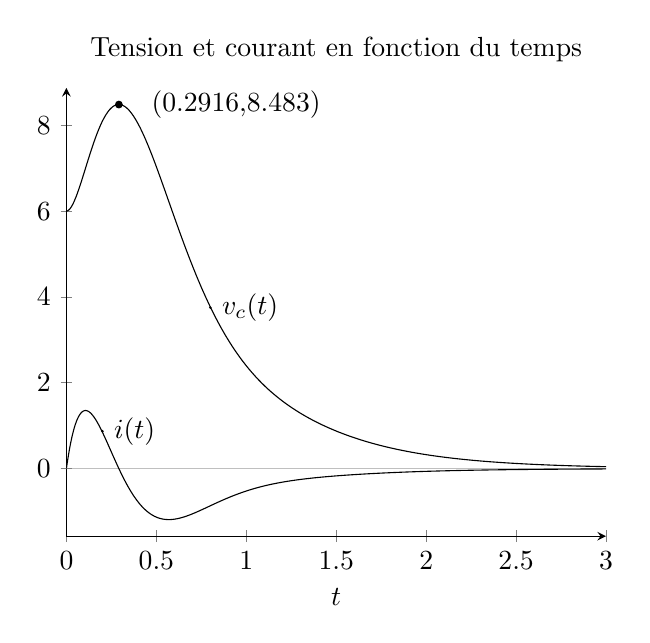
\begin{tikzpicture}
\begin{axis}[
    title = Tension et courant en fonction du temps,
    extra y ticks       = 0,
    extra y tick labels = ,
    extra y tick style  = { grid = major },
    axis lines = left,
    xlabel = \(t\),
    ylabel = %{\(y(t)\)}
    ,
    enlarge y limits=0.04,
]
% Plot de la tension
\addplot [
    domain=0:3, 
    samples=500, 
    color=black,
    ] {e^(-5*x)*((-198/17)*cos(deg(5*x))-(78/17)*sin(deg(5*x))) + (300/17)*e^(-2*x)};
\node[label={0:{$\ \ $(0.2916,8.483)}},circle,fill,inner sep=1pt] at (axis cs:0.2916,8.483) {};
\node[label={0:{$v_c(t)$}},circle,fill,inner sep=0pt] at (axis cs:0.8,3.75) {};

% Plot du courant
\addplot [
    domain=0:3, 
    samples=500, 
    color=black,
    ] {e^(-5*x)*((60/17)*cos(deg(5*x))+(138/17)*sin(deg(5*x))) -(60/17)*e^(-2*x)};
\node[label={0:{$i(t)$}},circle,fill,inner sep=0pt] at (axis cs:0.2,0.87) {};
\end{axis}
\end{tikzpicture}
\end{center}

d) La tension maximale est obtenue lorsque $v_c'(t)=0$. On utilise la fonction
solve de la Ti :
\begin{gather*}
    \solve\prt{0=\dv{v_c(t)}{t},t} \\
    \implies t=0.2916
\end{gather*}

En mettant cette valeur de temps dans $v_c(t)$, on trouve que la tension maximale
est de 8.483 Volts. Le courant à cet instant là est nul, car :
\begin{align*}
    i(0.2916) = C\dv{v_c(t)}{t}\vert_{t=0.2916}
\end{align*}

or :
\begin{align*}
    \dv{v_c(t)}{t}\vert_{t=0.2916} = 0 \implies i(0.2916) = 0
\end{align*}
